\chapter{Strain B-scan Images}\label{images}

This appendix shows the 2D B-scan images for the six different processing techniques at different fit and lateral resolutions. It is important to analyse the image as a whole, rather than just looking at sensitivity and image resolution, because artefacts may manifest in areas outside of those used to calculate these parameters. Also, these images provide a more intuitive understanding of the affect of changing the resolution parameters. The following B-scan images were produced:

\begin{table}[h!]
	\centering
	\begin{tabular}{|c|c||l|l|}
		\hline
		FR ($\mu m$) & LR ($\mu m$) & Image & Comments \\
		\hline
		\hline
		40 & 0 & \autoref{fr40_lr0} & Good resolution due to small fit value, \\
		& & & however corruption by noise degrades \\
		& & & sensitivity. \\
		\hline
		100 & 0 & \autoref{fr100_lr0} & Over-smoothed fit resolution, to demonstrate \\
		& & & trade-off between sensitivity and \\
		& & & resolution. \\
		\hline
		40 & 20 & \autoref{fr40_lr20} & Applying lateral smoothing to increase \\
		& & & sensitivity for small fit resolution. \\
		\hline
		70 & 20 & \autoref{fr70_lr20} & Small lateral smoothing filter applied \\
		& & & at the standard processing fit \\
		& & & resolution. \\
		\hline
		40 & 40 & \autoref{fr40_lr40} & Equal lateral and 'axial' (fit) smoothing\\
		\hline
	\end{tabular}
\end{table}

\begin{figure}[h]
	\centering
    \begin{subfigure}{0.49\textwidth}
    	\centering
        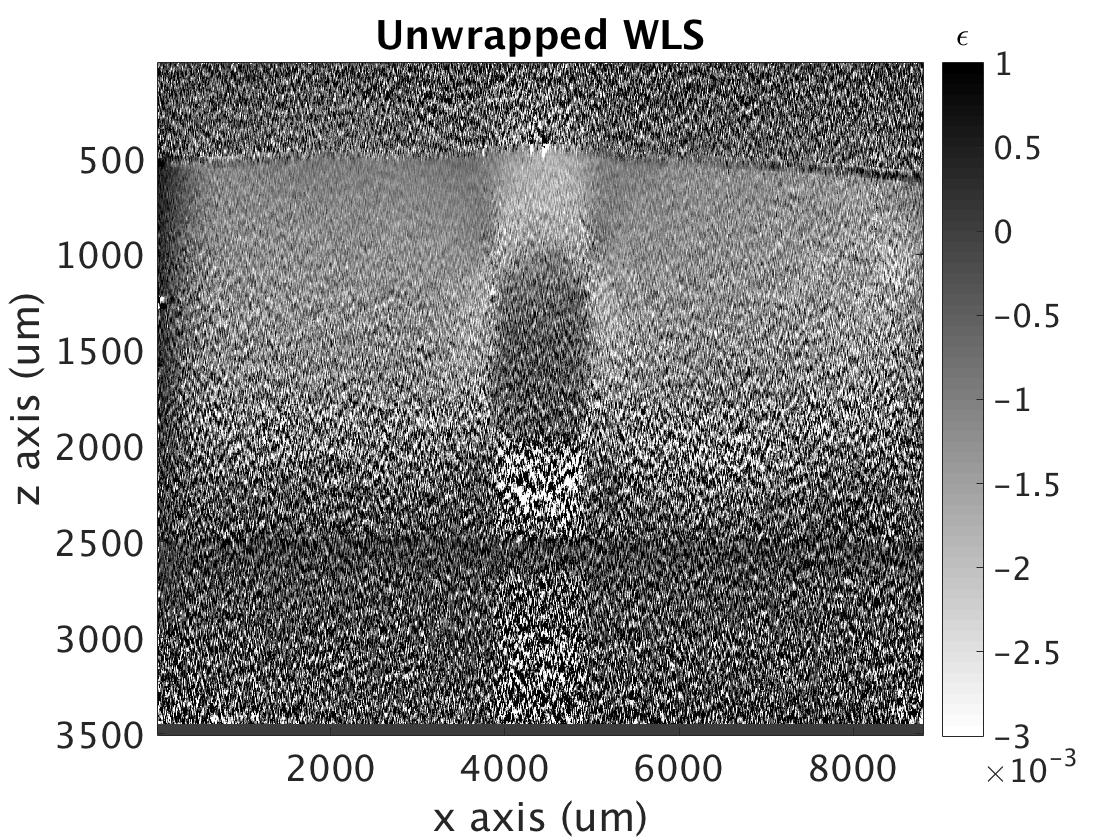
\includegraphics[width=\textwidth]{appendix_figs/wls_fr40_lr0.png}
    \end{subfigure}
    \begin{subfigure}{0.49\textwidth}
    	\centering
        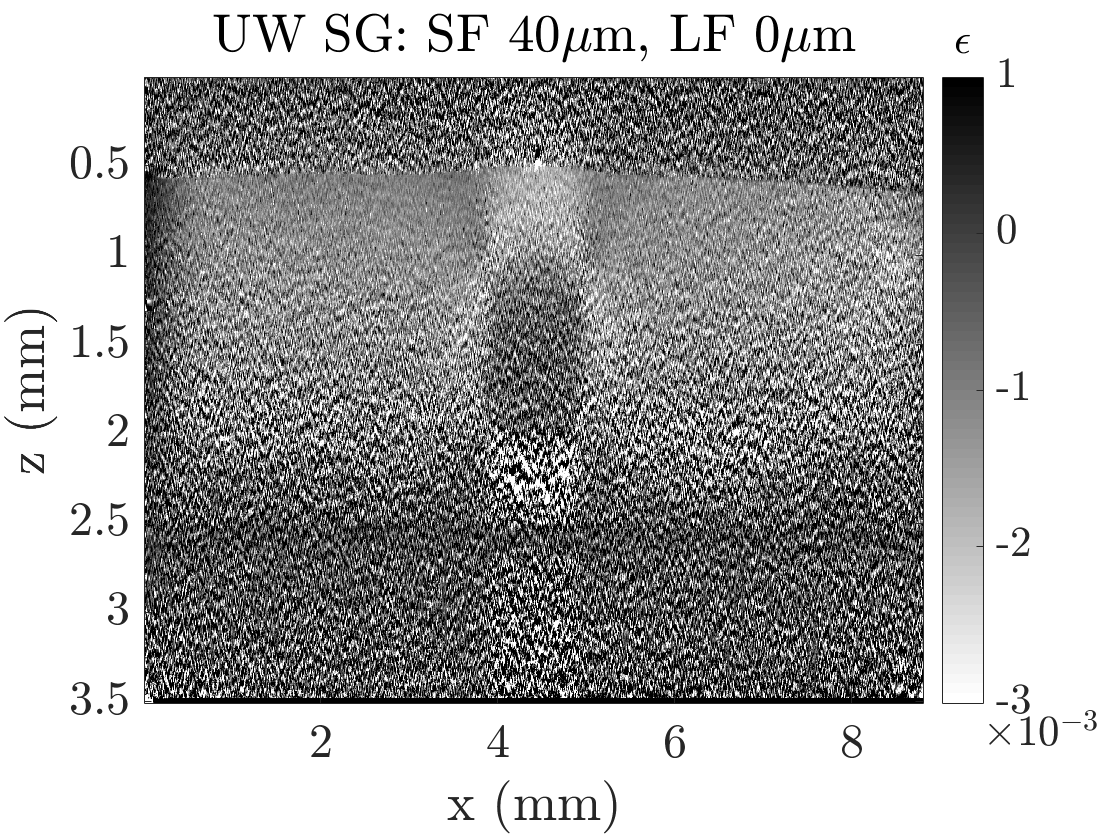
\includegraphics[width=\textwidth]{appendix_figs/uwsg_fr40_lr0.png}
    \end{subfigure}
    \\
    \begin{subfigure}{0.49\textwidth}
    	\centering
        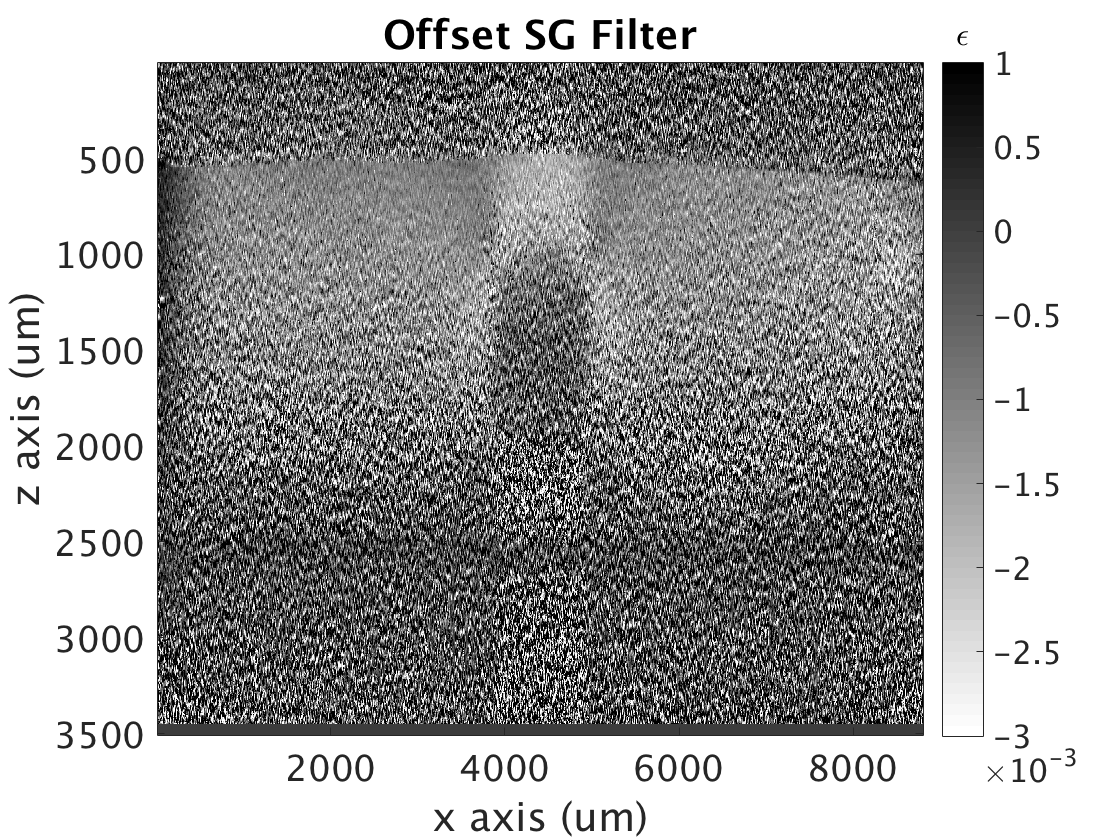
\includegraphics[width=\textwidth]{appendix_figs/posg_fr40_lr0.png}
    \end{subfigure}
    \begin{subfigure}{0.49\textwidth}
    	\centering
        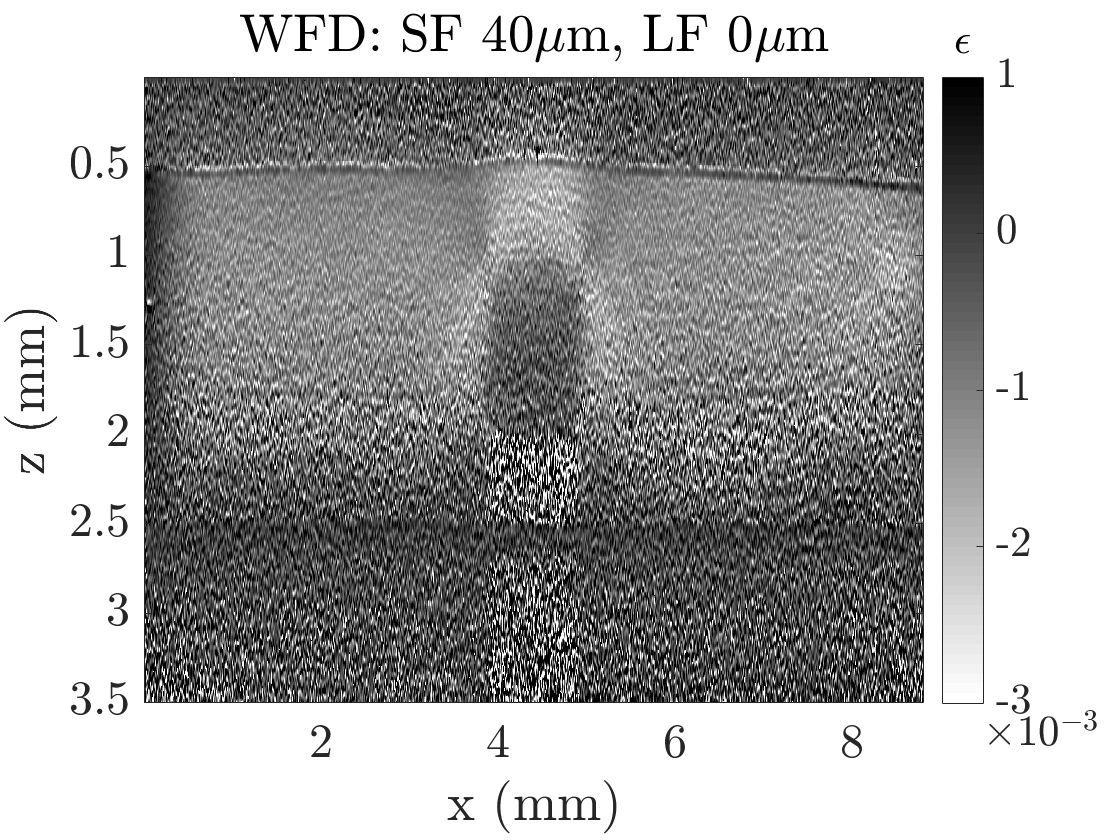
\includegraphics[width=\textwidth]{appendix_figs/wfd_fr40_lr0.png}
    \end{subfigure}
    \\
    \begin{subfigure}{0.49\textwidth}
    	\centering
        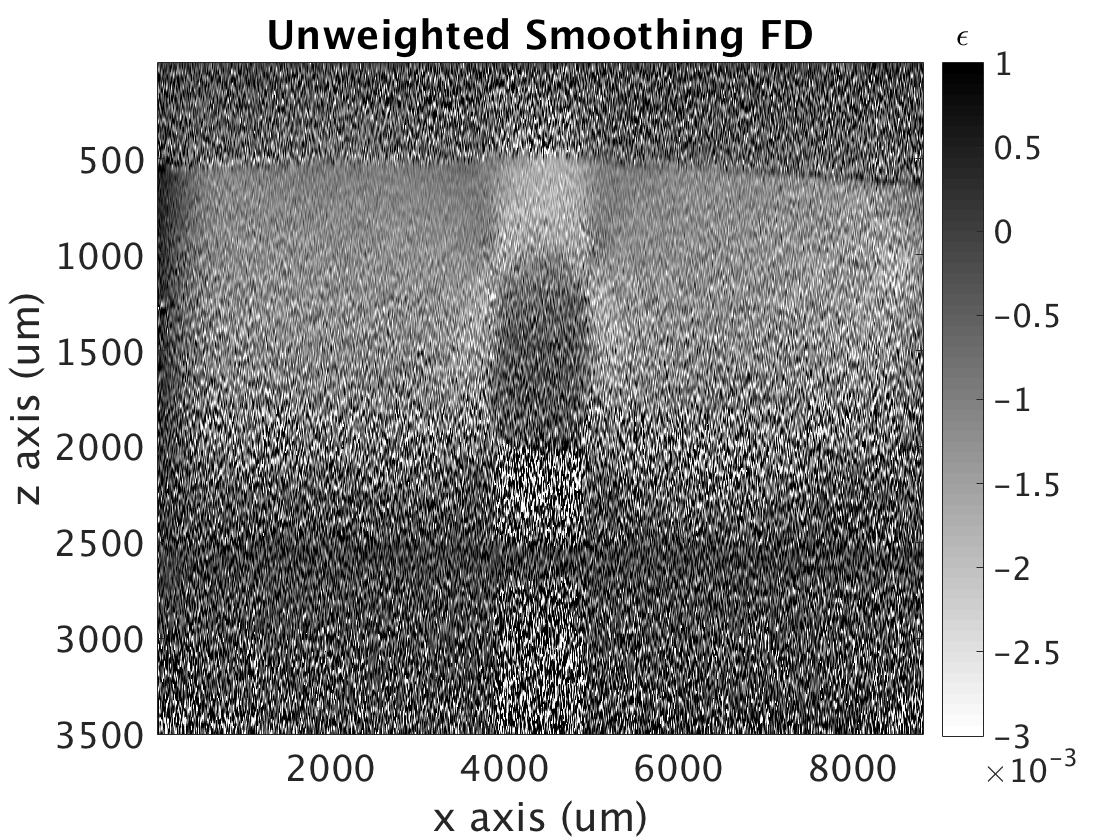
\includegraphics[width=\textwidth]{appendix_figs/uwfd_fr40_lr0.png}
    \end{subfigure}
    \begin{subfigure}{0.49\textwidth}
    	\centering
        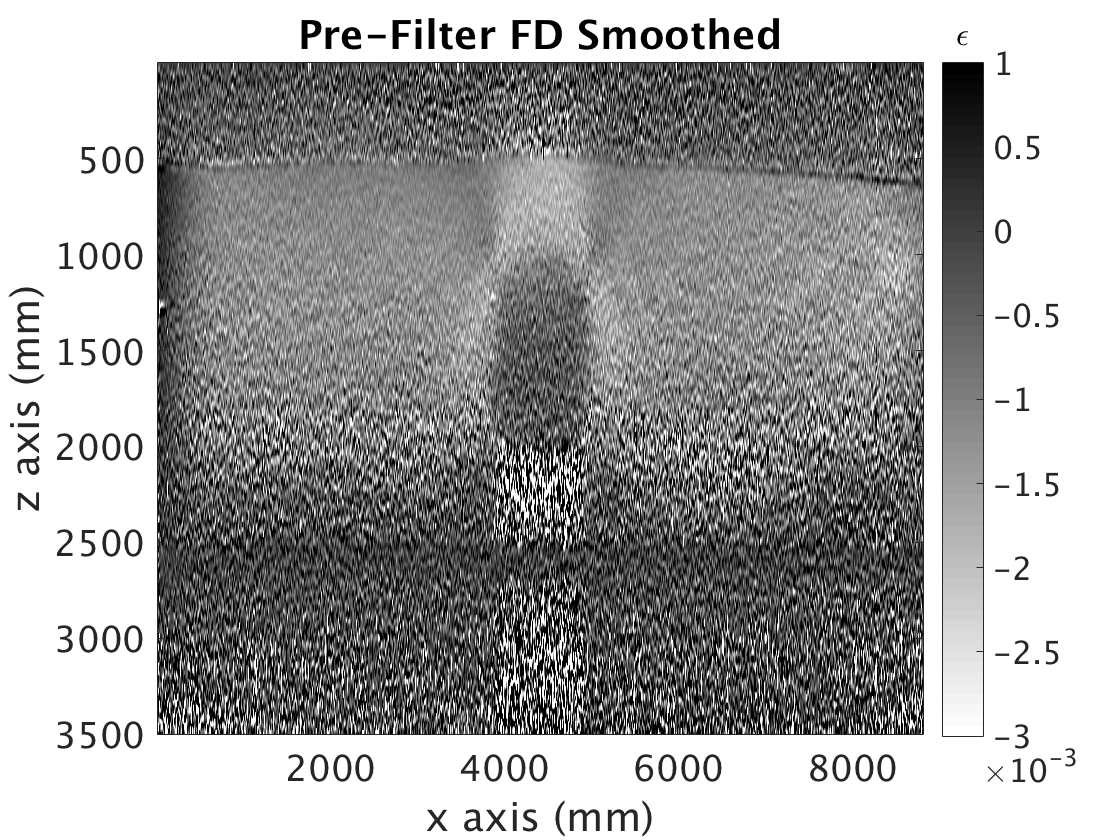
\includegraphics[width=\textwidth]{appendix_figs/fdsm_fr40_lr0.png}
    \end{subfigure}    
    \caption{Strain B-scans for the different strain estimation techniques, taken at a lower fit resolution of $40\mu m$, with no lateral smoothing.}
	\label{fr40_lr0}
\end{figure}

\begin{figure}[h]
	\centering
    \begin{subfigure}{0.49\textwidth}
    	\centering
	    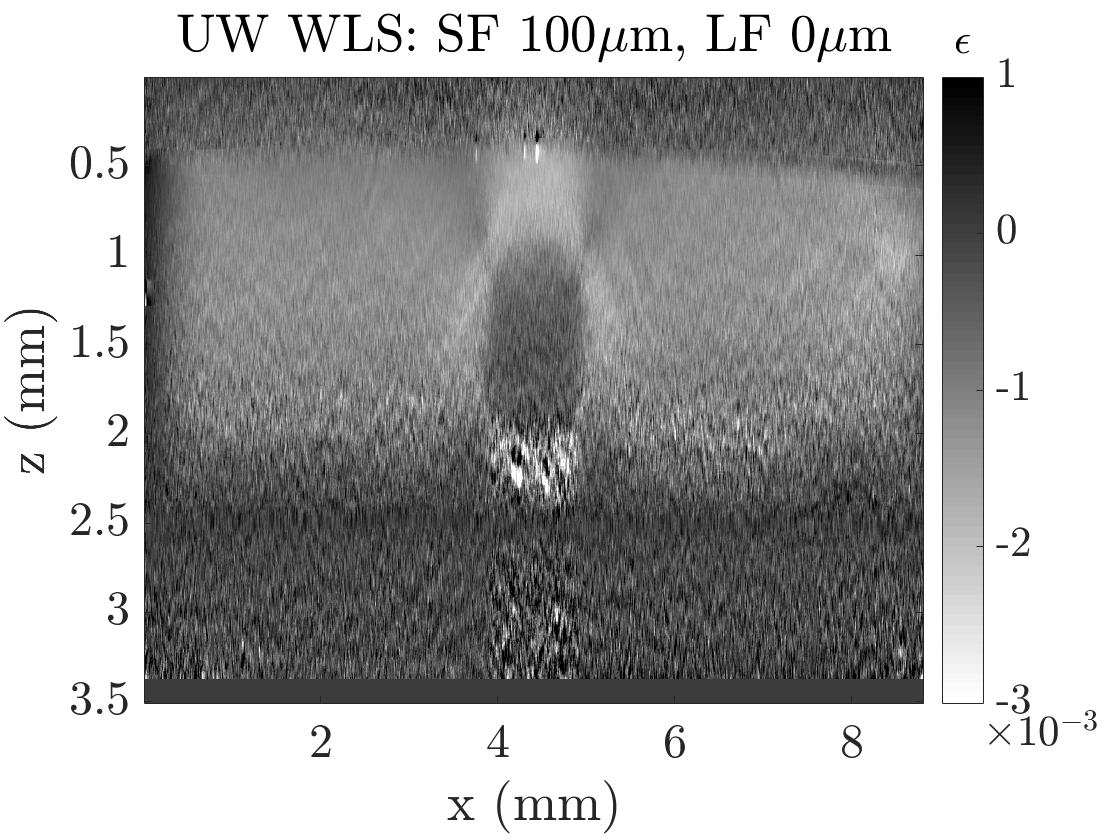
\includegraphics[width=\textwidth]{appendix_figs/wls_fr100_lr0.png}
    \end{subfigure}
    \begin{subfigure}{0.49\textwidth}
    	\centering
        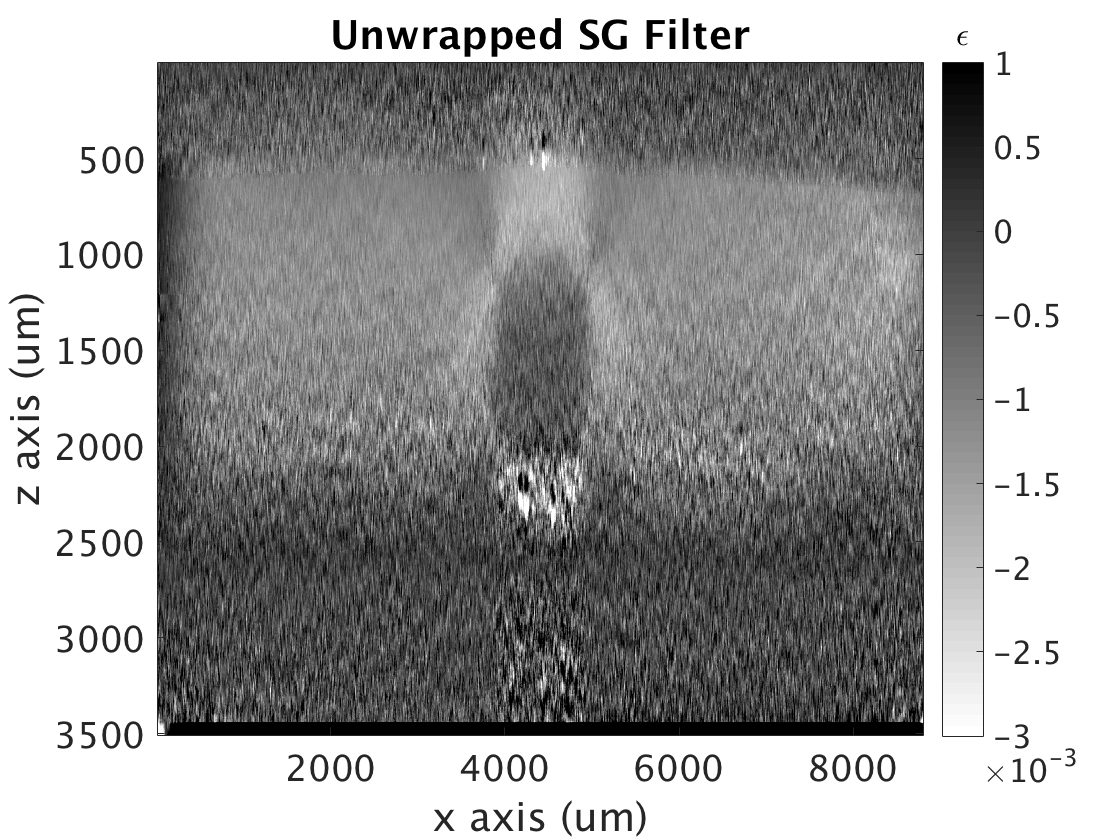
\includegraphics[width=\textwidth]{appendix_figs/uwsg_fr100_lr0.png}
    \end{subfigure}
    \\
    \begin{subfigure}{0.49\textwidth}
    	\centering
        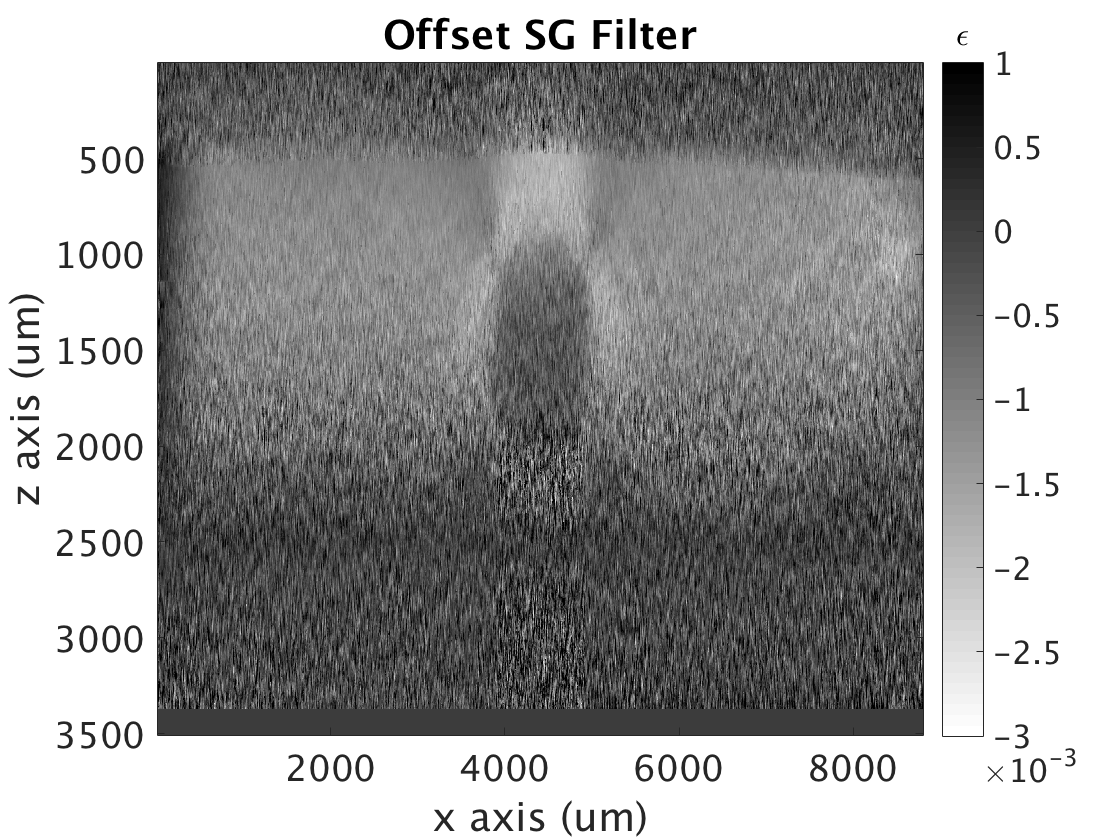
\includegraphics[width=\textwidth]{appendix_figs/posg_fr100_lr0.png}
    \end{subfigure}
    \begin{subfigure}{0.49\textwidth}
    	\centering
        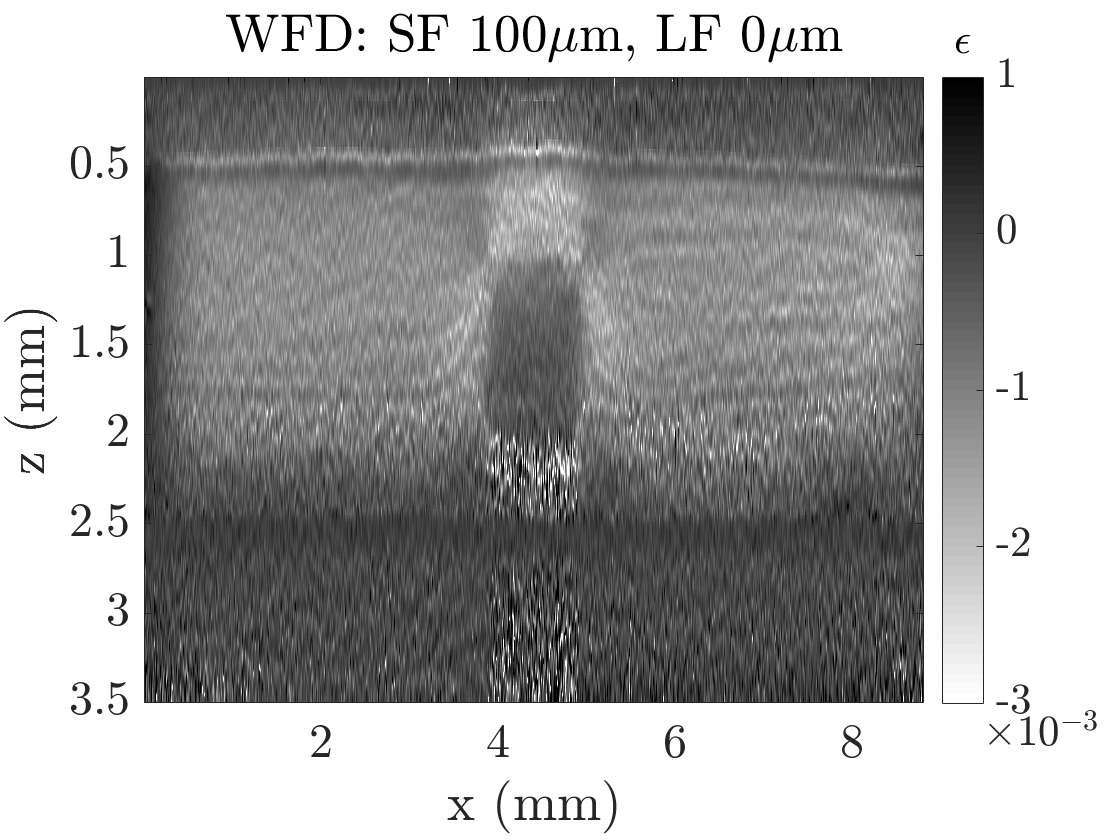
\includegraphics[width=\textwidth]{appendix_figs/wfd_fr100_lr0.png}
    \end{subfigure}
    \\
    \begin{subfigure}{0.49\textwidth}
    	\centering
        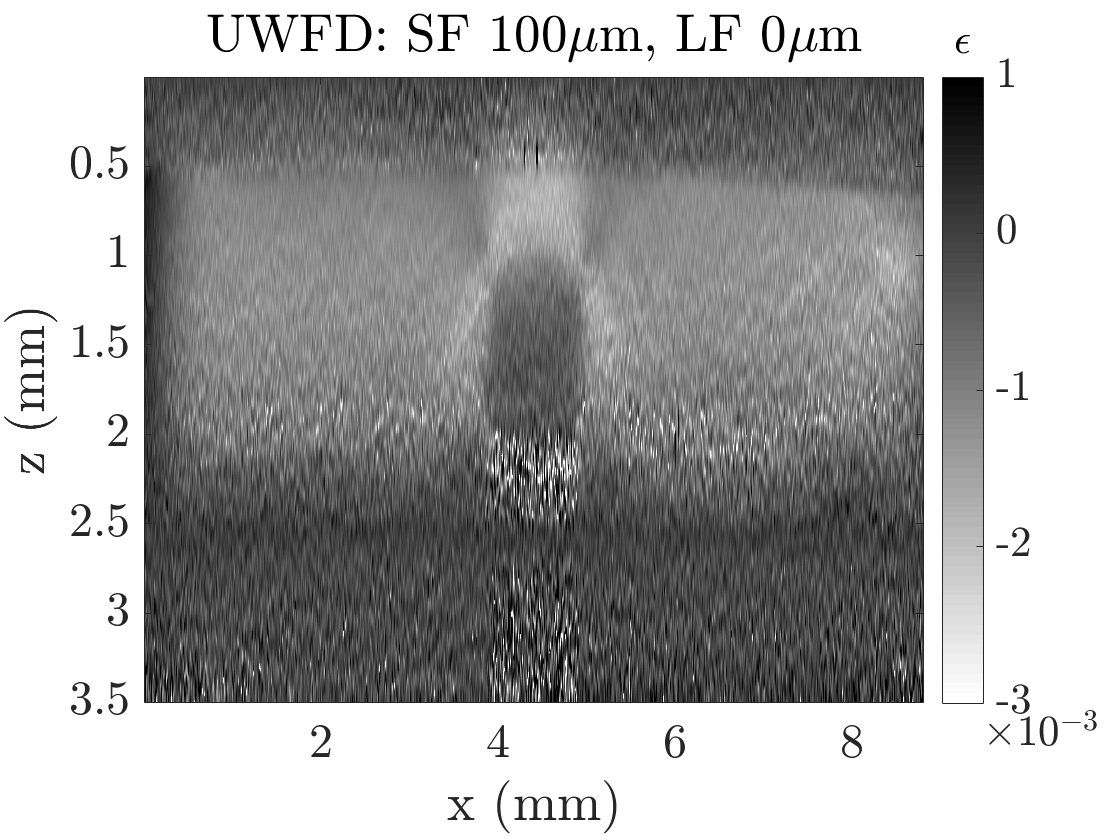
\includegraphics[width=\textwidth]{appendix_figs/uwfd_fr100_lr0.png}
    \end{subfigure}
    \begin{subfigure}{0.49\textwidth}
    	\centering
        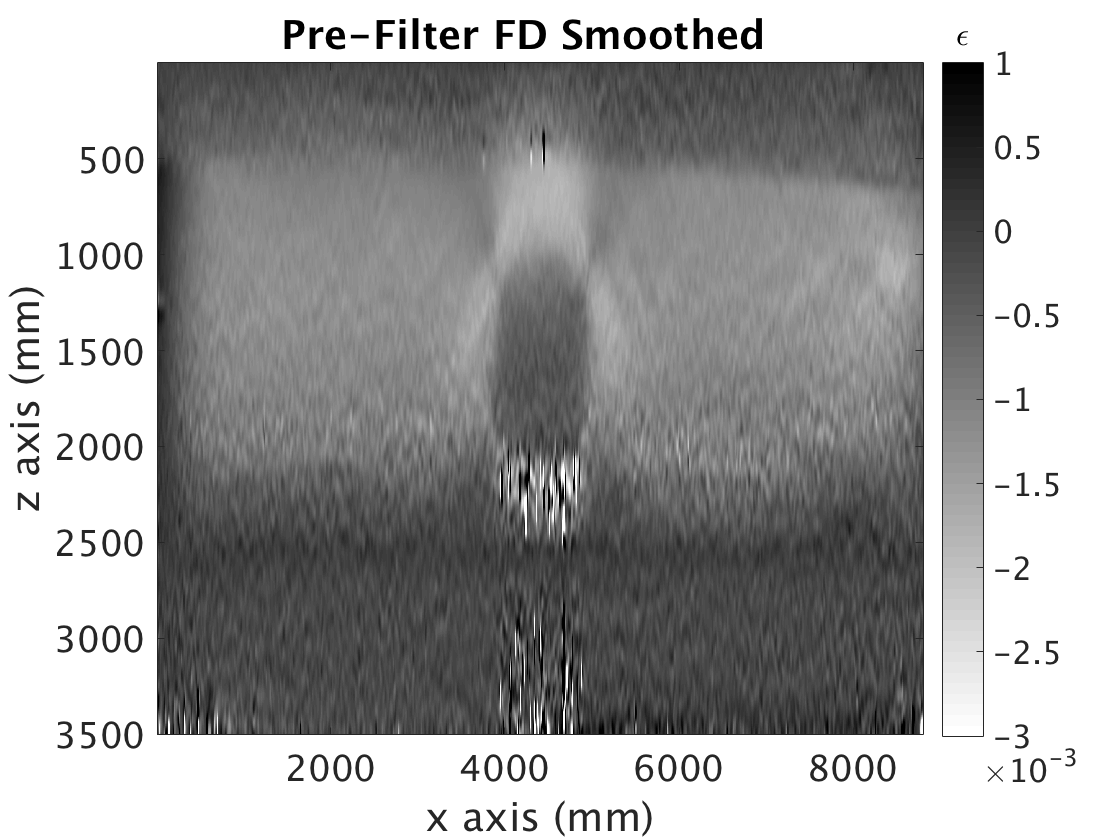
\includegraphics[width=\textwidth]{appendix_figs/fdsm_fr100_lr0.png}
    \end{subfigure}    
    \caption{Strain B-scans for the different strain estimation techniques, taken at a higher than average fit resolution of $100\mu m$, with no lateral smoothing.}
	    \label{fr100_lr0}
\end{figure}

\begin{figure}[h]
	\centering
    \begin{subfigure}{0.49\textwidth}
    	\centering
        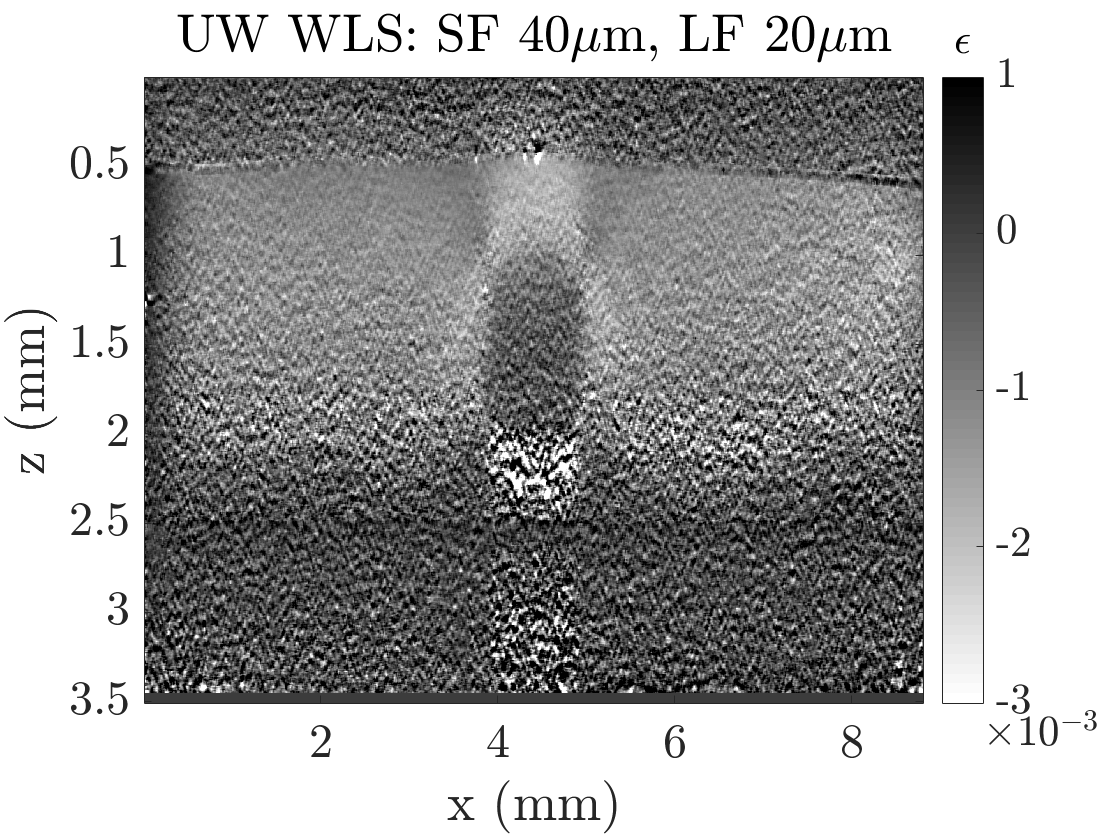
\includegraphics[width=\textwidth]{appendix_figs/wls_fr40_lr20.png}
    \end{subfigure}
    \begin{subfigure}{0.49\textwidth}
    	\centering
        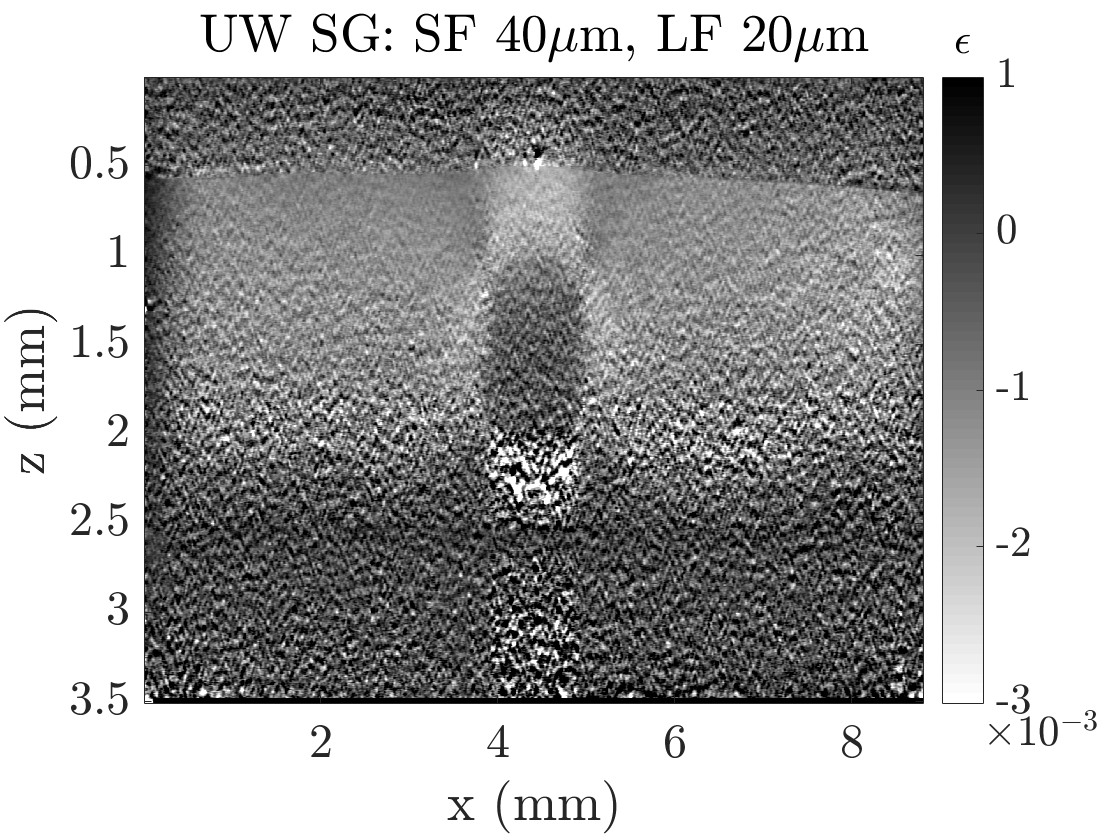
\includegraphics[width=\textwidth]{appendix_figs/uwsg_fr40_lr20.png}
    \end{subfigure}
    \\
    \begin{subfigure}{0.49\textwidth}
    	\centering
        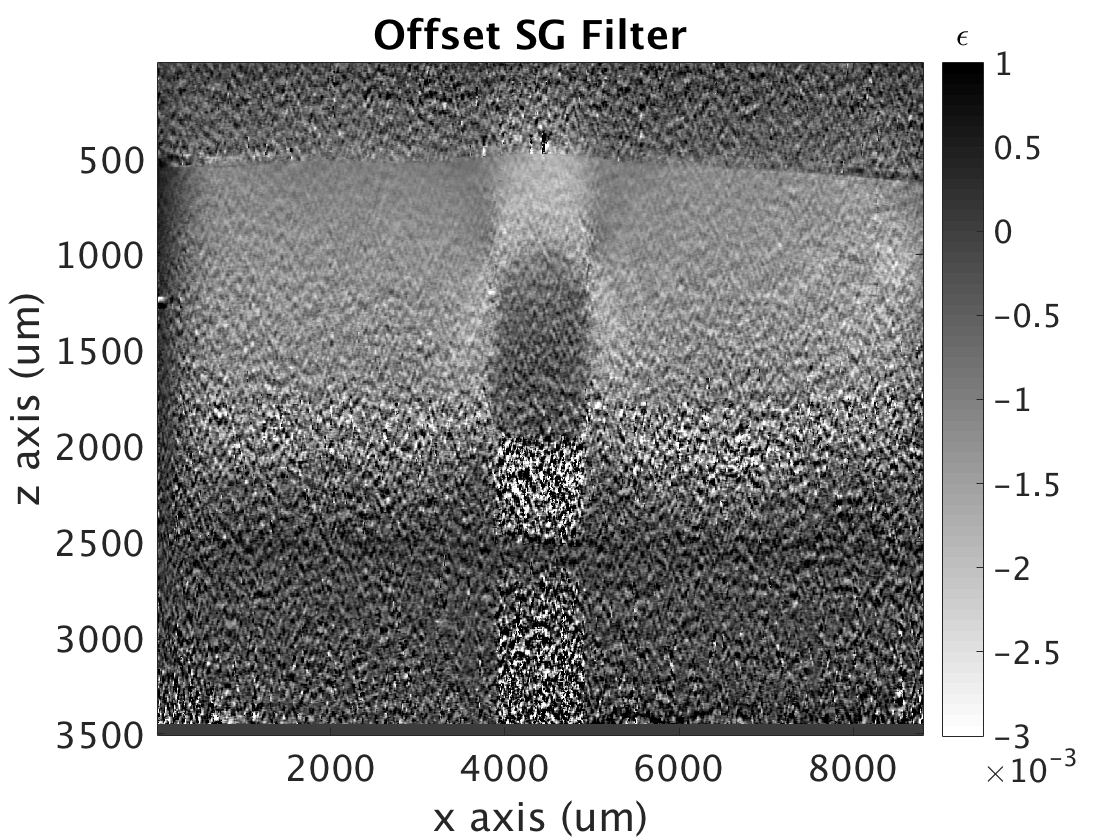
\includegraphics[width=\textwidth]{appendix_figs/posg_fr40_lr20.png}
    \end{subfigure}
    \begin{subfigure}{0.49\textwidth}
    	\centering
        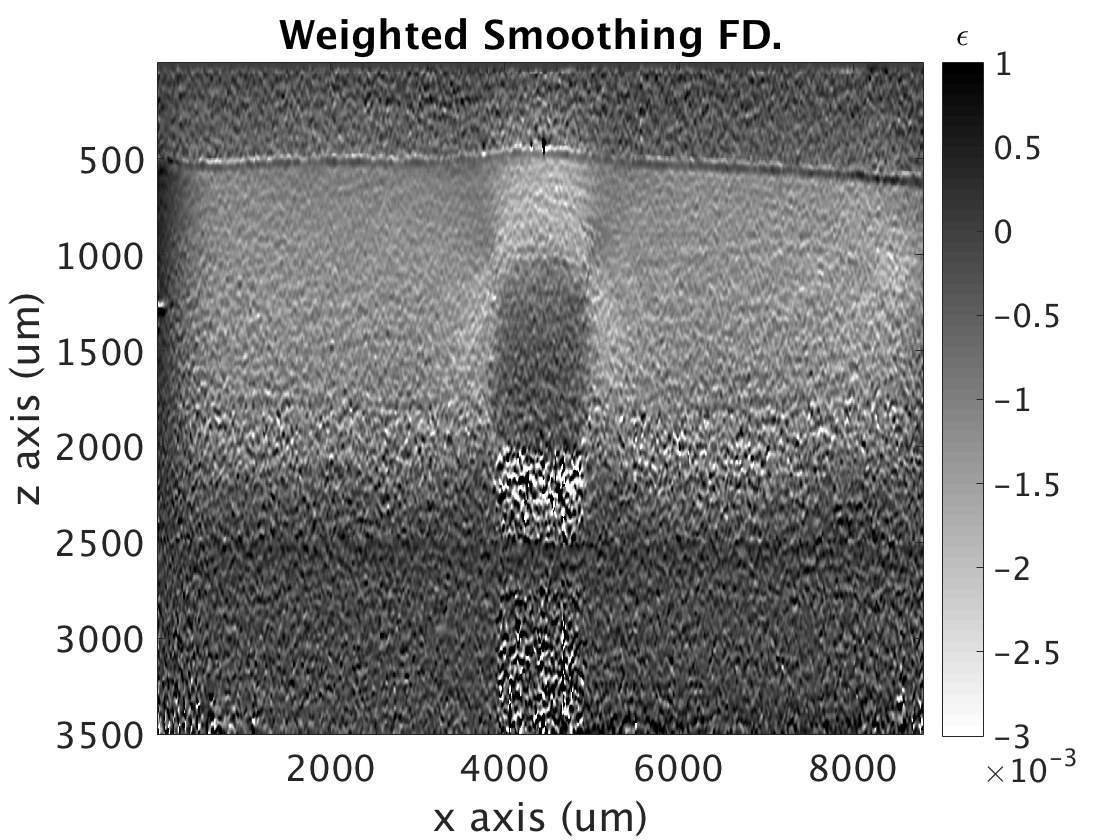
\includegraphics[width=\textwidth]{appendix_figs/wfd_fr40_lr20.png}
    \end{subfigure}
    \\
    \begin{subfigure}{0.49\textwidth}
    	\centering
        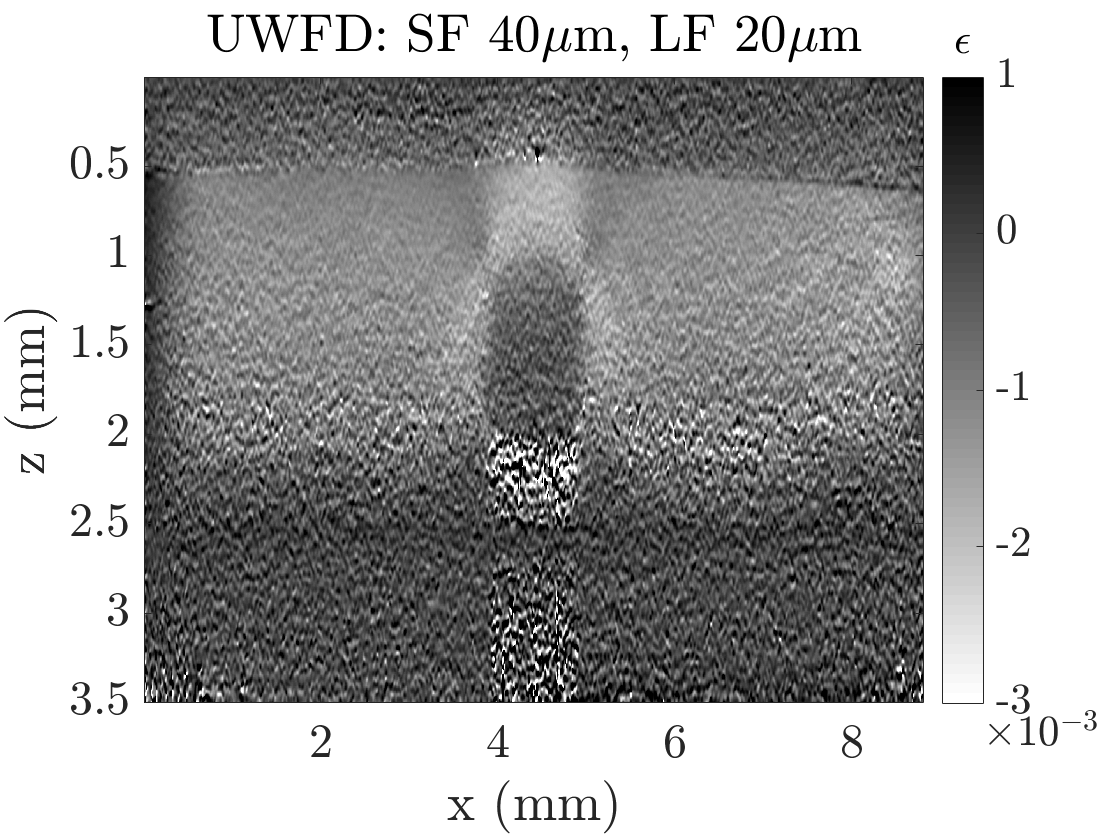
\includegraphics[width=\textwidth]{appendix_figs/uwfd_fr40_lr20.png}
    \end{subfigure}
    \begin{subfigure}{0.49\textwidth}
    	\centering
        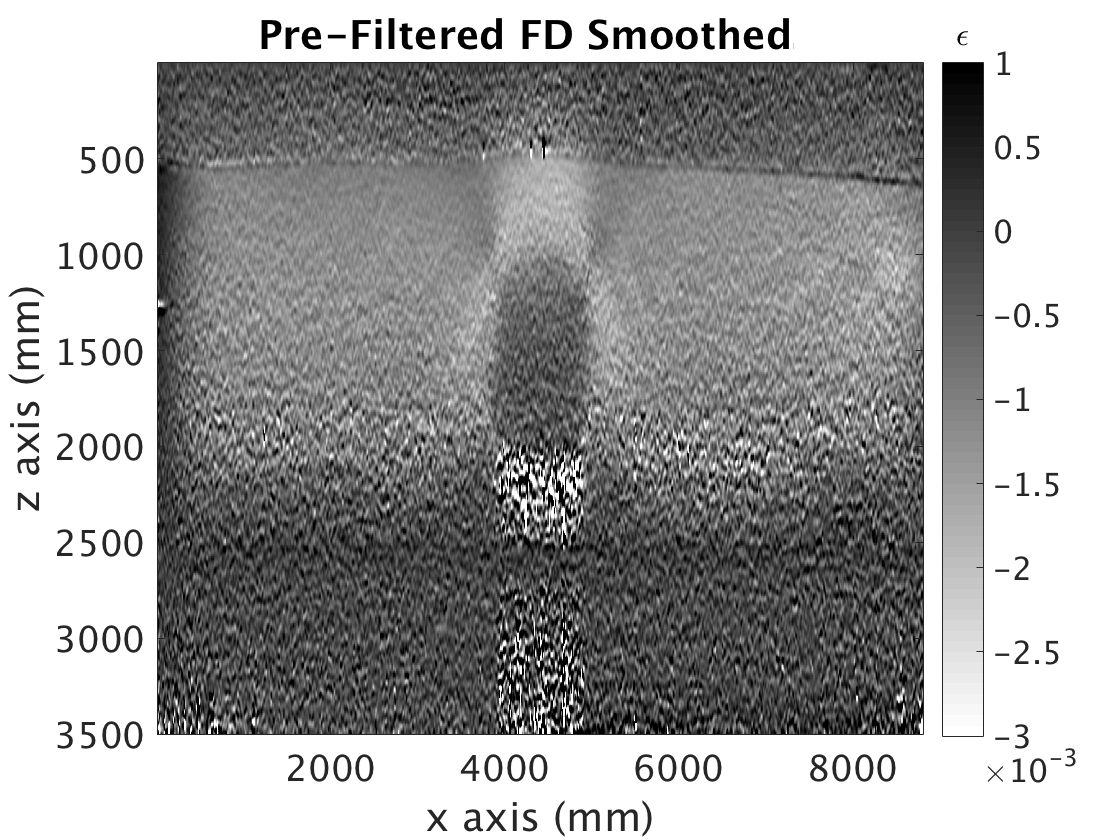
\includegraphics[width=\textwidth]{appendix_figs/fdsm_fr40_lr20.png}
    \end{subfigure}    
    \caption{Strain B-scans for the different strain estimation techniques, taken at a lower fit resolution of $40\mu m$, with lateral smoothing of $20 \mu m$ resolution.}
	\label{fr40_lr20}
\end{figure}


\begin{figure}[h]
	\centering
    \begin{subfigure}{0.49\textwidth}
    	\centering
        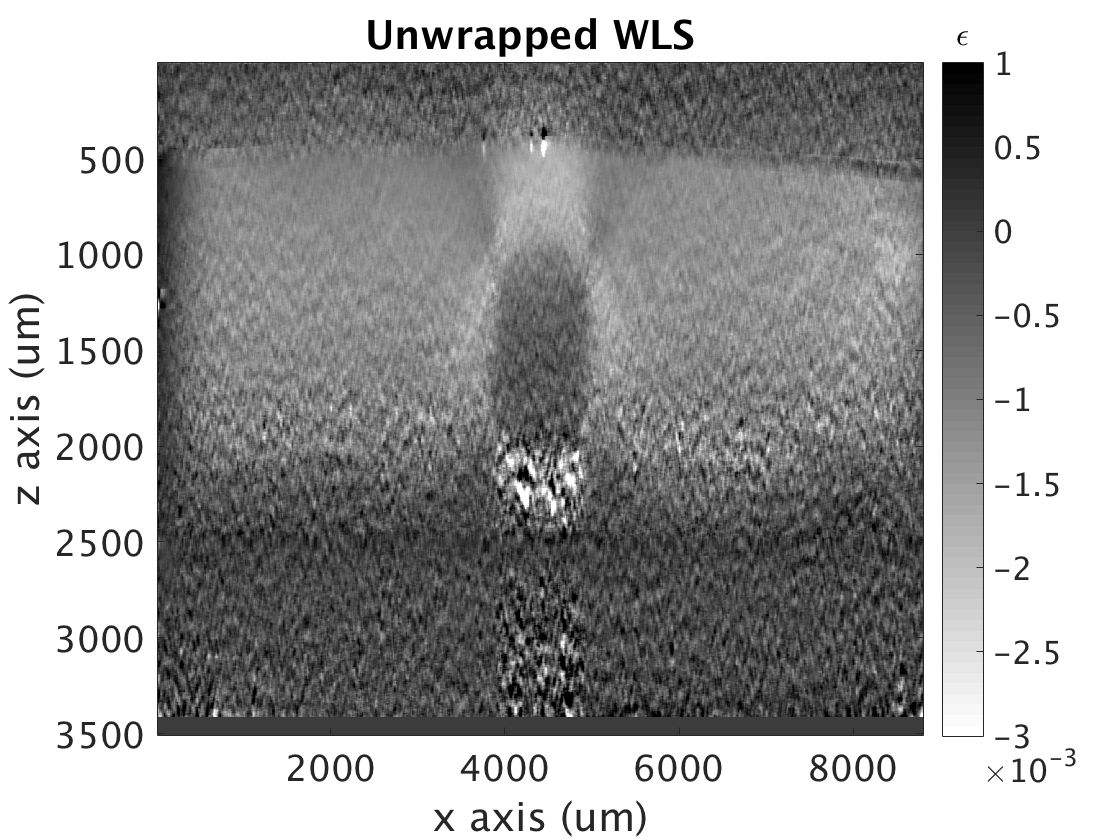
\includegraphics[width=\textwidth]{appendix_figs/wls_fr70_lr20.png}
    \end{subfigure}
    \begin{subfigure}{0.49\textwidth}
    	\centering
        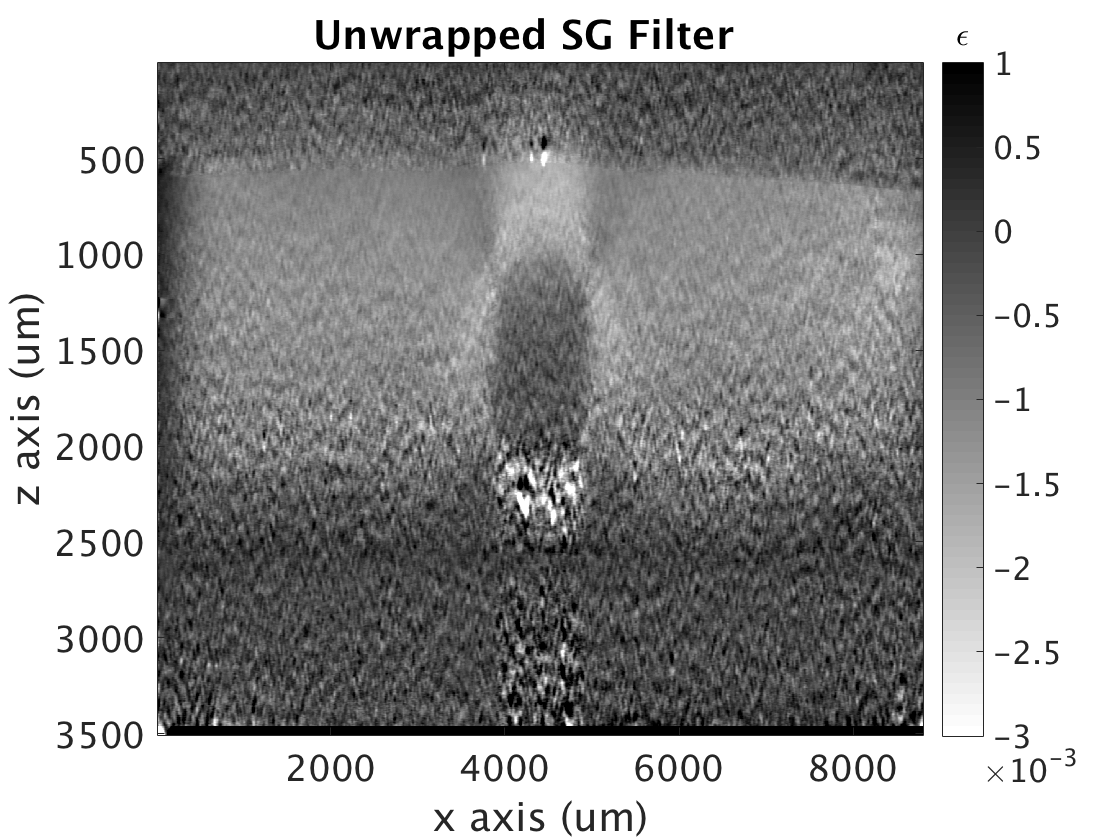
\includegraphics[width=\textwidth]{appendix_figs/uwsg_fr70_lr20.png}
    \end{subfigure}
    \\
    \begin{subfigure}{0.49\textwidth}
    	\centering
        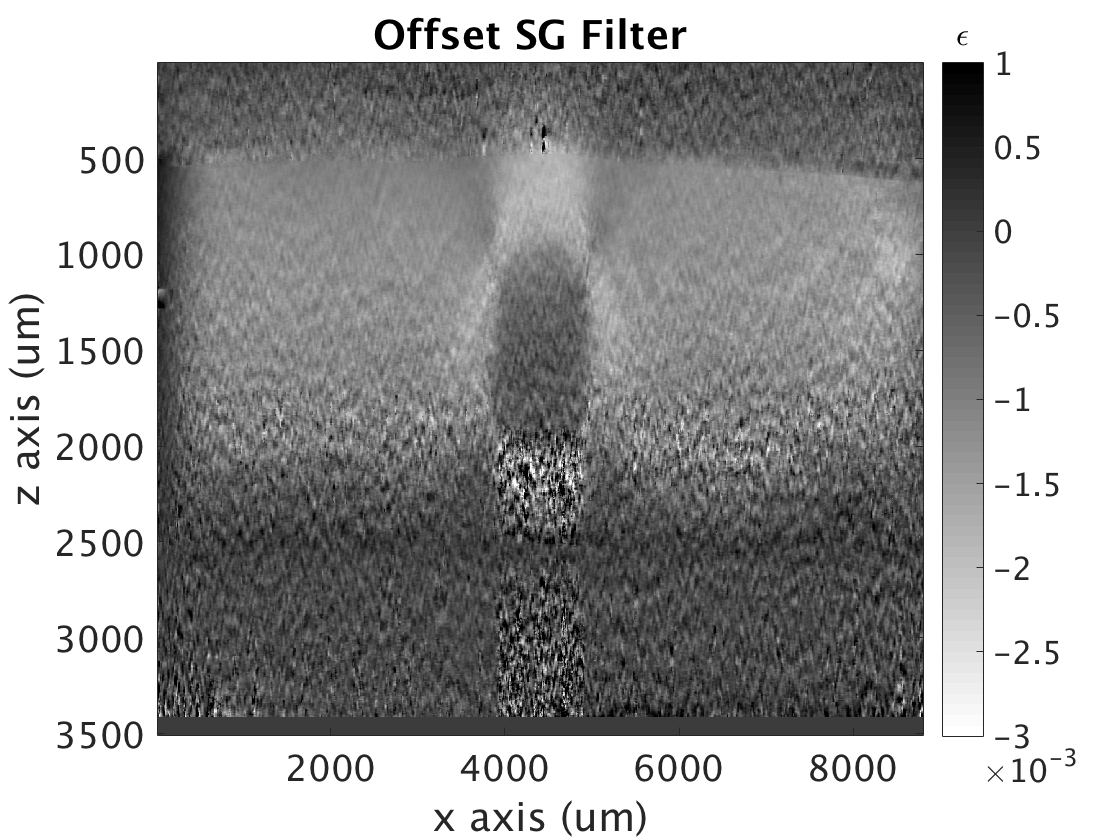
\includegraphics[width=\textwidth]{appendix_figs/posg_fr70_lr20.png}
    \end{subfigure}
    \begin{subfigure}{0.49\textwidth}
    	\centering
        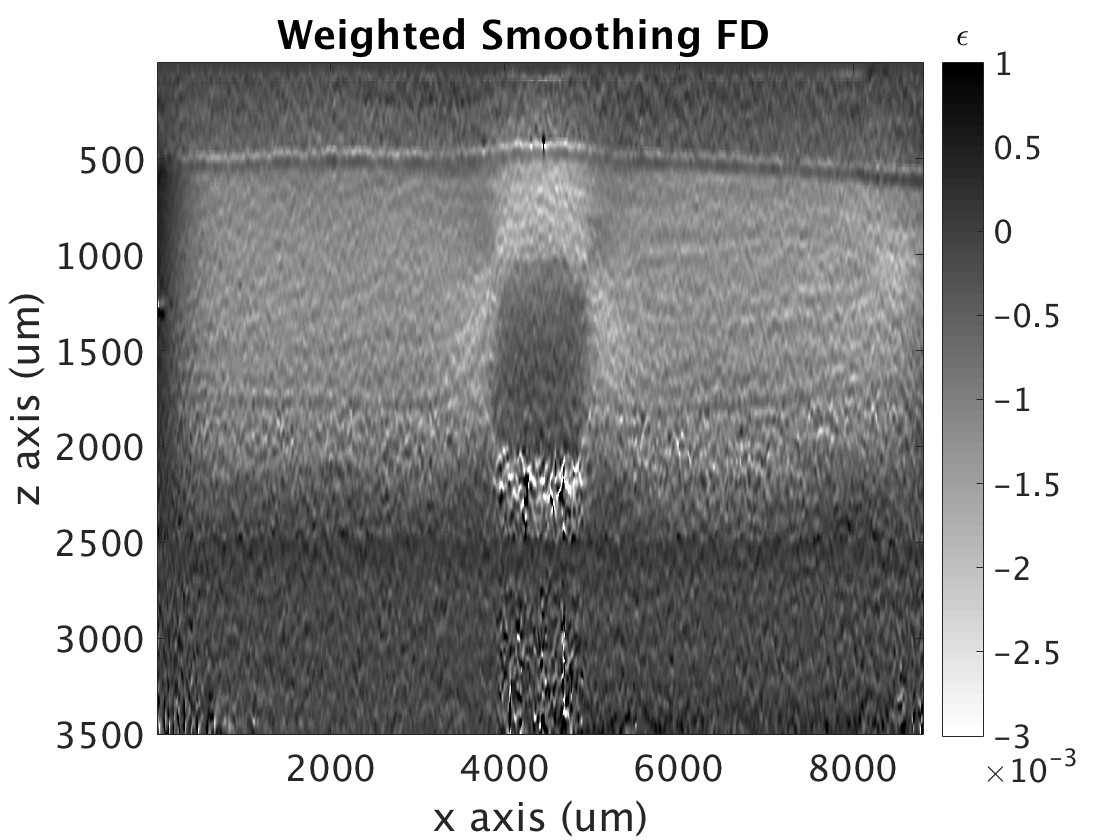
\includegraphics[width=\textwidth]{appendix_figs/wfd_fr70_lr20.png}
    \end{subfigure}
    \\
    \begin{subfigure}{0.49\textwidth}
    	\centering
        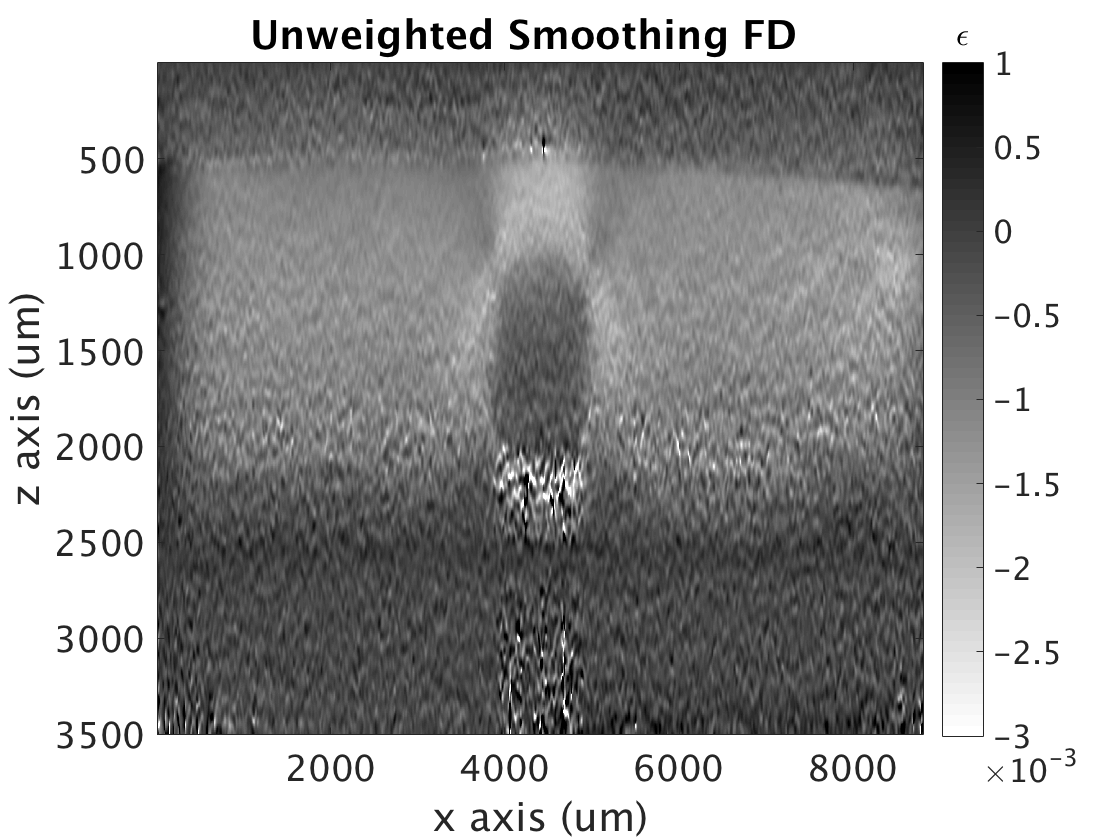
\includegraphics[width=\textwidth]{appendix_figs/uwfd_fr70_lr20.png}
    \end{subfigure}
    \begin{subfigure}{0.49\textwidth}
    	\centering
        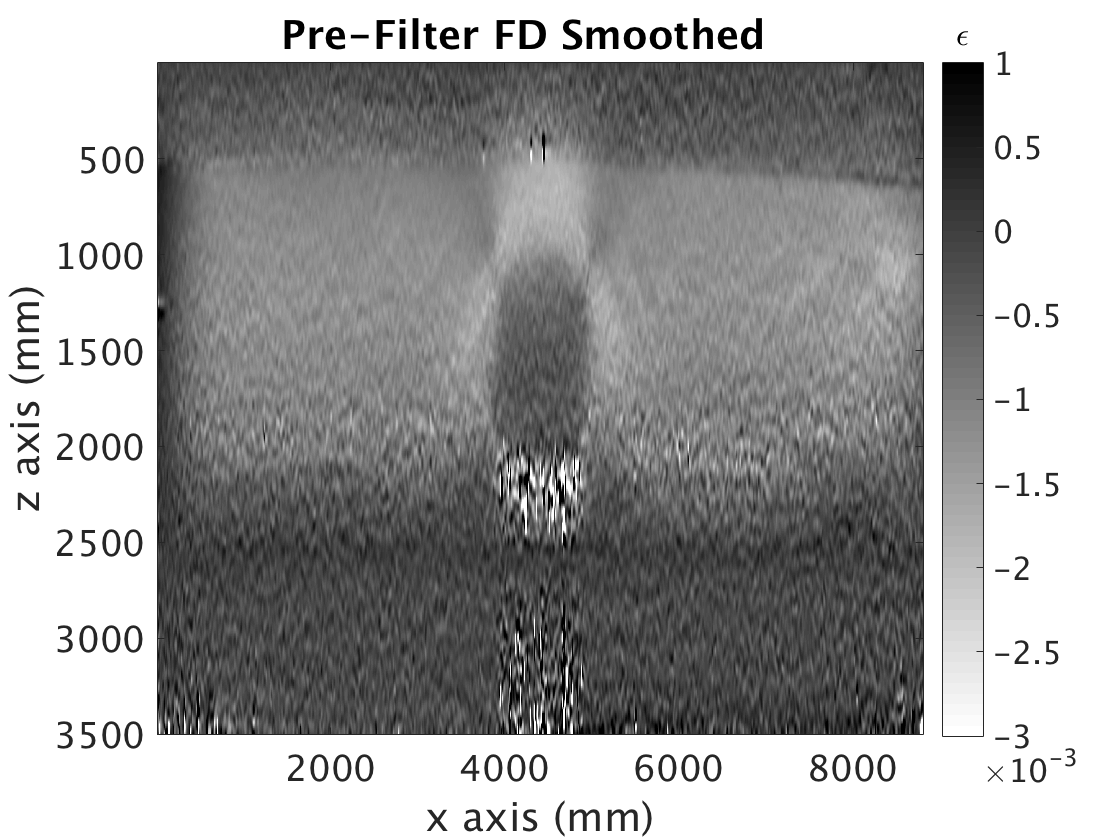
\includegraphics[width=\textwidth]{appendix_figs/fdsm_fr70_lr20.png}
    \end{subfigure}    
    \caption{Strain B-scans for the different strain estimation techniques, at the standard fit resolution ($70 \mu m$ but with added lateral smoothing of resolution $20 \mu m$.}
    \label{fr70_lr20}
\end{figure}

\begin{figure}[h]
	\centering
    \begin{subfigure}{0.49\textwidth}
    	\centering
        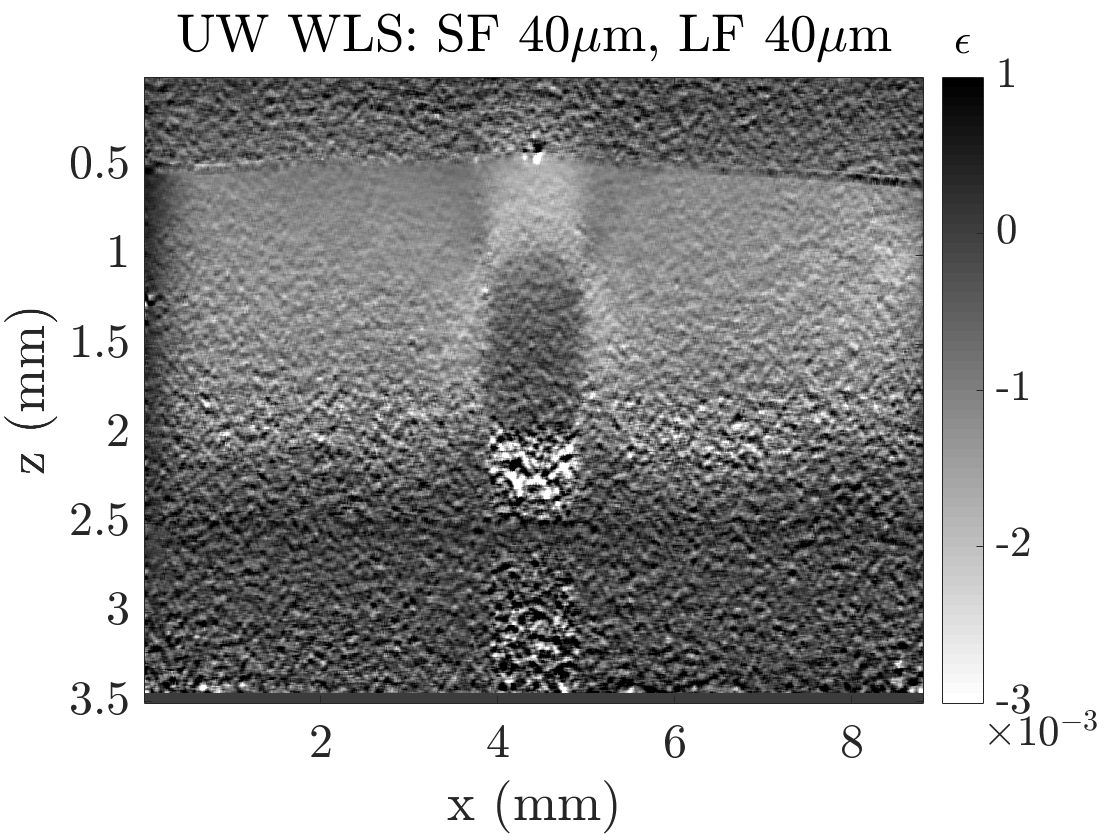
\includegraphics[width=\textwidth]{appendix_figs/wls_fr40_lr40.png}
    \end{subfigure}
    \begin{subfigure}{0.49\textwidth}
    	\centering
        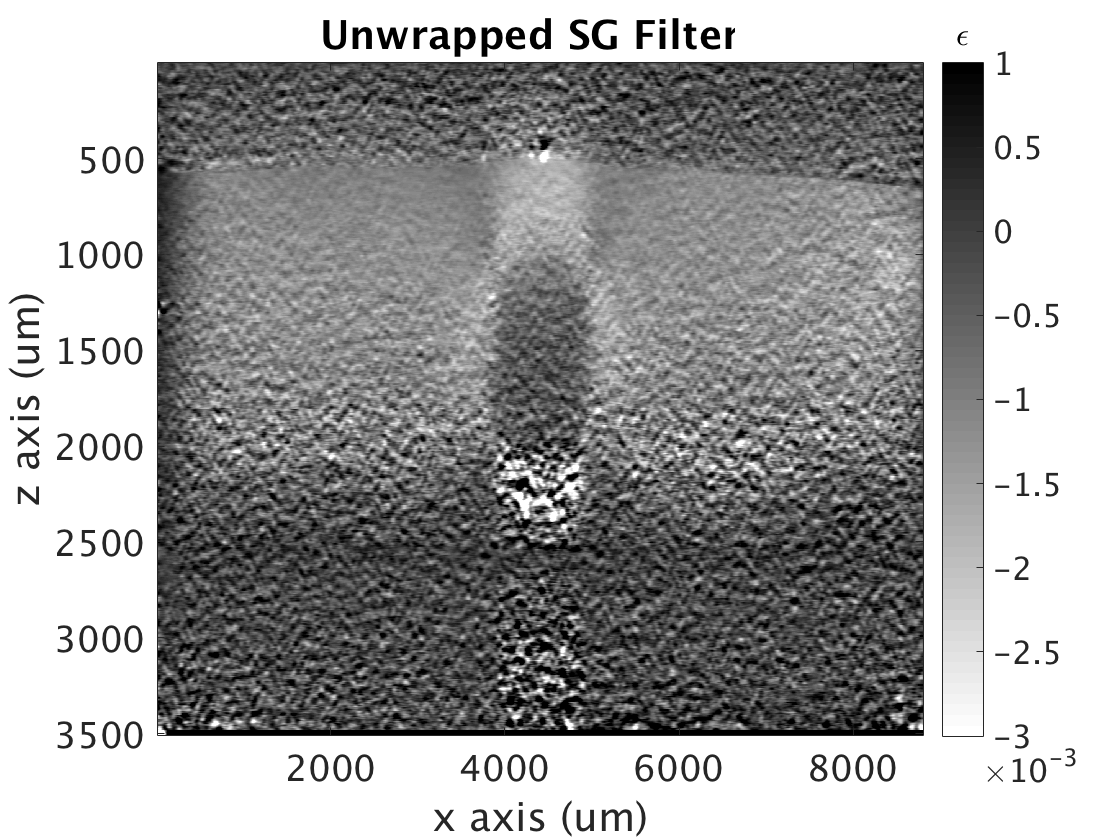
\includegraphics[width=\textwidth]{appendix_figs/uwsg_fr40_lr40.png}
    \end{subfigure}
    \\
    \begin{subfigure}{0.49\textwidth}
    	\centering
        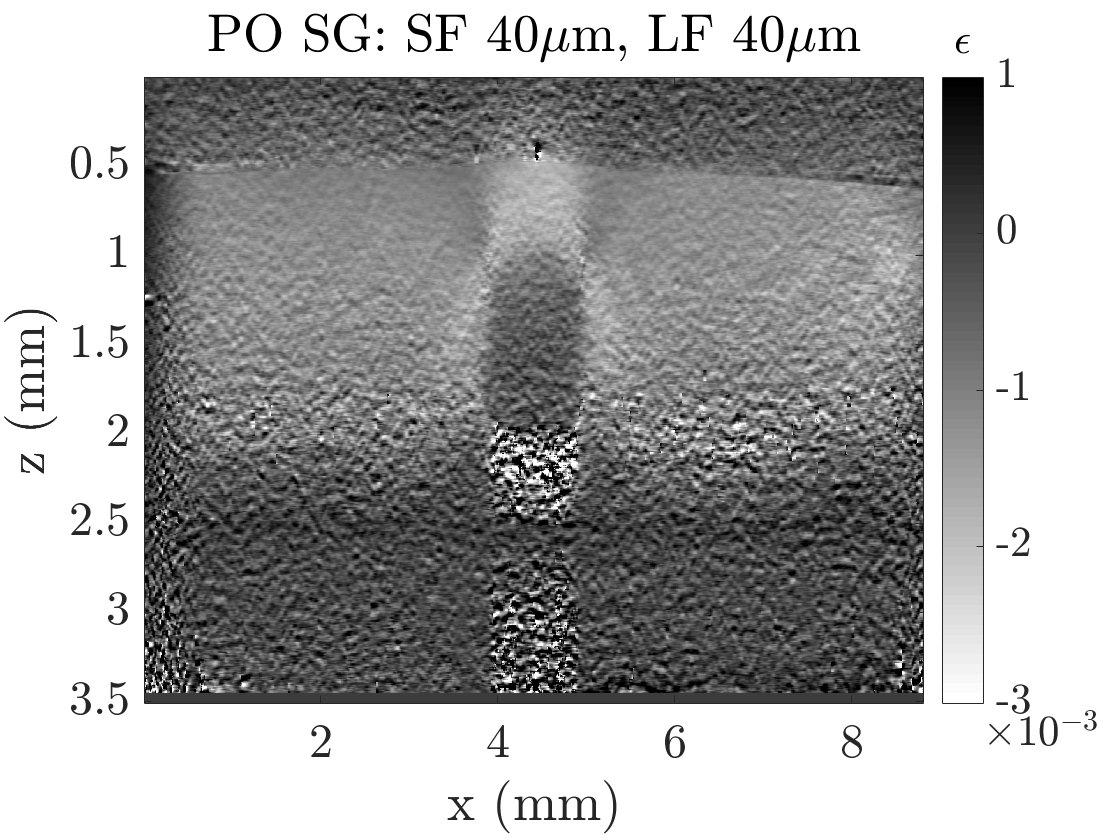
\includegraphics[width=\textwidth]{appendix_figs/posg_fr40_lr40.png}
    \end{subfigure}
    \begin{subfigure}{0.49\textwidth}
    	\centering
        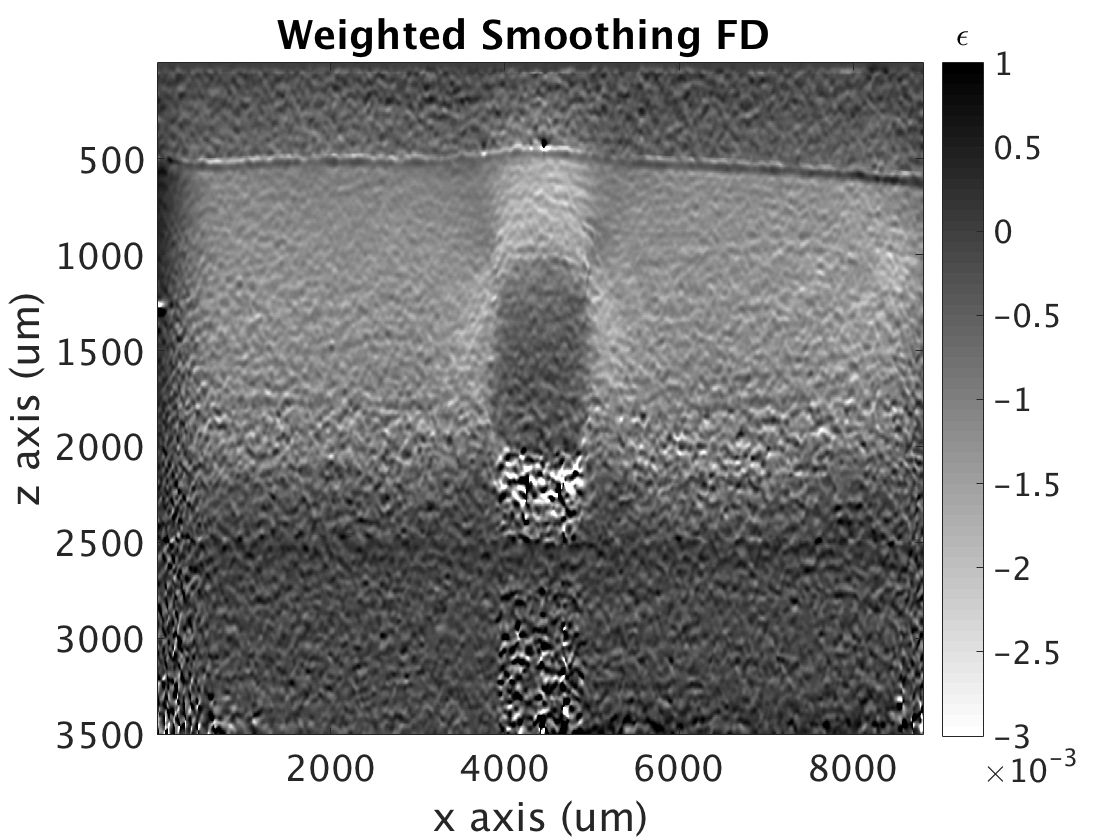
\includegraphics[width=\textwidth]{appendix_figs/wfd_fr40_lr40.png}
    \end{subfigure}
    \\
    \begin{subfigure}{0.49\textwidth}
    	\centering
        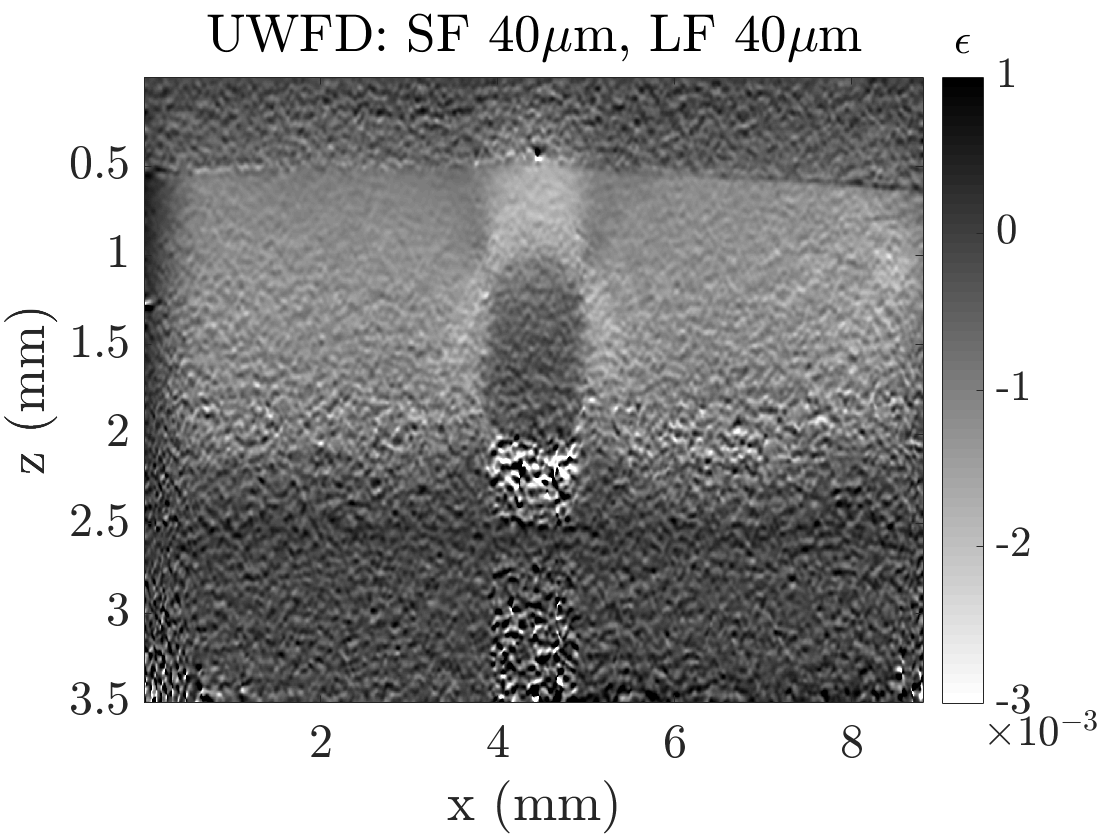
\includegraphics[width=\textwidth]{appendix_figs/uwfd_fr40_lr40.png}
    \end{subfigure}
    \begin{subfigure}{0.49\textwidth}
    	\centering
        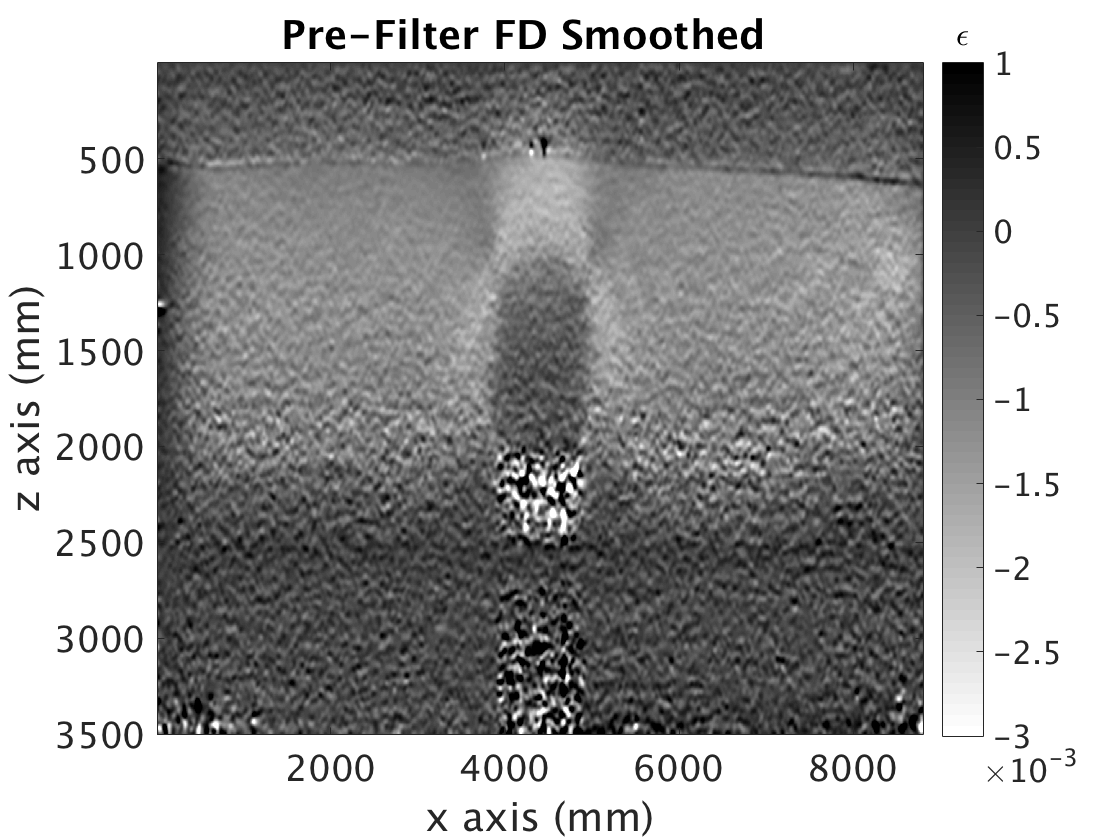
\includegraphics[width=\textwidth]{appendix_figs/fdsm_fr40_lr40.png}
    \end{subfigure}    
    \caption{Strain B-scans for the different strain estimation techniques, taken at a lower fit resolution of $40\mu m$, with a higher lateral smoothing of $40 \mu m$ resolution.}
	\label{fr40_lr40}
\end{figure}

